\title{Лекции по моделированию}
\chapter{Лекция 1}
\section{Расписание и формат обучения}
Приём лабораторных:\\
Среда:
15:40 - 17:15, 237л\\
17:25 - 19:00 237л\\

Суббота:
13:50 - 15:25 243л\\
15:40 - 17:15 243л\\

Модули:\\
М1: 5 неделя, минимум 12 баллов, максимум 20 баллов, одна лабораторная\\
М2: 12 неделя, минимум 12 баллов, максимум 20 баллов, две лабораторные\\
М3: 17 неделя, минимум 18 баллов, максимум 30 баллов, одна лабораторная\\

Сдано больше двух лабораторных - автомат на экзамене.

\section{Комментарии к первой лабораторной работе}
\begin{equation}
\begin{cases}
u'(x) = x^{2} + u^{2}
u(0) = 0
\end{cases}
\end{equation}

Результат:
\begin{itemize}
\item значения для $x \in [0, x_{max}]$ с заданным шагом h
\item приближения Пикара с 1 по 4 порядок
\item до второго знака после запятой - точность
\item график функции в интервале $[-x_{max}, x_{max}]$
\end{itemize}

\section{Погрешности и устойчивость}
Погрешности, возникающие при моделировании:
\begin{itemize}
\item Погрешность модели
\item Погрешность метода
\item Погрешность исходных данных
\item Погрешность округления
\end{itemize}

Устойчивость - задача называется устойчивой (корректной), если решение единственно и устойчиво по входным данныхм. Плохо обусловленная задача: $\delta y = C \delta x, C >> 0$

\section{Модели на основе ОДУ}
Все дополнительные условия заданы в одной точке - задача Коши.\\
Все дополнительные условия заданы в разных точках - краевая задача.\\

Задача Коши:\\
$u'(x) = f(x, u)$\\
$u(\xi) = \eta$\\

Решением данной задачи является сведение уравнения к производным первого порядка при помощи замены переменных:\\
$u^{n}(x) = f(x, u, u', ..., u^{n-2}, u^{n-1})$\\
$u^{(k)} = u_{k}$\\

\begin{equation}
\begin{cases}
u'_{k}=u^{(k+1)}=u_{k+1}, 0 \leqslant k \leqslant n - 2\\
u'_{n} = f(x, u_{0}, u_{1}, u_{2}, ..., u_{n-1})
\end{cases}
\end{equation}
$u_{0} \equiv u$\\
$u_{k}(\xi) = \eta_{k}, 0 \leqslant k \leqslant n - 1$\\

Методы решения:\\
\begin{itemize}
\item Аналитические
\item Приближенно аналитические
\item Численные
\end{itemize}

Для оценки точности численных методов можно использовать правило Рунге, заключающееся в том, что если мы рассчитаем функцию с шагом $h$ и $h/2$, то точность в $x_{i}$ будет выражаться как: $\frac{|y_{i, h} - y_{i, h/2}|}{2^{p} - 1}$, где p - порядок точности.

\section{Явные методы Рунге-Кутта}
$u'(x) = f(x, u)$\\
$u(\xi) = \eta$\\
$a \leqslant x \leqslant b$\\

\begin{figure}[H]
	\center{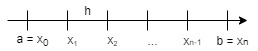
\includegraphics[scale=1.5]{a_0}}
	\caption{Значения на числовой прямой}
\end{figure}

$w_{N} = \{x_{i} : a = x_{0} < x_{1} ... < x_{N}\}$\\
$w_{n} = \{x_{i}: x_{i} = a + ih, i = \overline{0, N}\}$\\
$y_{i} \rightarrow y(x_{i})$\\

Сходимость разностного решения к точному на отрезке:\\
$\forall x_{i} \in [a, b]: |y_{i} - u_{i}| \rightarrow 0, h \rightarrow 0 (i \rightarrow \infty)$

\subsection{Метод Эйлера (p=1)}
$u_{i+1} = u_{i} + h_{i} \cdot u'_{i} + \frac{h^{2}}{2!}u''_{i}+ \frac{h^{3}}{3!}u'''_{i} + ...$\\
здесь $u'_{i} = u'(x_{i}); u''_{i} = u''(x_{i}) ...$\\
$y_{i+1} = y_{i} + h \cdot f(x_{i}, u_{i})$, если $|y_{i} - u_{i}| = o(h^{2})$, при $h \rightarrow 0$, то метод имеет p-й порядок точности.

\subsection{Численный метод Рунге-Кутта (p=2)}
$u_{i+1} = u_{i} + h u'_{i} + \frac{h^{2}}{2}u''_{i} + ...$\\
$u'_{i} = f_{i} = f(x_{i}, u_{i})$\\
$u''_{i} = (u'_{i}) = \frac{d}{dx}f = f'_{x_{i}} + f'_{u_{i}} \cdot f_{i}$\\
$y_{i+1} = y_{i} + h f_{i} + \frac{h^{2}}{2}(f'_{x_{i}} + f'_{y_{i}} \cdot f_{i}), (p=2), (2)$\\ 
$u''{i} = \frac{f(x + \gamma h, y + \delta h) - f(x, y)}{\Delta x}$\\
$y_{i+1} = y_{i} + h f_{i} + \frac{h^{2}}{2}(\frac{f(x + \gamma h, y + \delta h) - f(x, y)}{\Delta x}) = y_{i} + h[\beta f(x_{i}, y_{i}) + \alpha f (x_{i} + \gamma h, y_{i} + \delta h)]$ (3)\\
$y_{i+1} = y_{i} + h[\beta f(x_{i} + y_{i}) + \alpha (f(x_{i}, y_{i}) + f'_{x}\gamma h + f'_{y} \delta h)] = y_{i} + h[(\alpha + \beta) f(x_{i}, y_{i}) + \alpha \gamma h f'_{x} + \alpha \delta h f'_{y}]$ (4)\\

Сравним (2) и (4):\\
\begin{equation}
\begin{cases}
\alpha + \beta = 1\\
\alpha \gamma = \frac{1}{2}\\
\alpha \delta = \frac{1}{2} f(x_{i}, y_{i})\\
\end{cases}
\end{equation}

\begin{equation}
\begin{cases}
\beta = 1 - \alpha\\
\gamma = \frac{1}{2\alpha}\\
\delta = \frac{1}{2\alpha} f(x_{i}, y_{i})\\
\end{cases}
\end{equation}

Из (3) видим, что:\\
$y_{i+1} = y_{i} + h[(1 - \alpha) f(x_{i}, y_{i}) + \alpha f(x_{i} + \frac{1}{2\alpha}h, y_{i} + \frac{h}{2\alpha}f(x_{i}, y_{i}))]$, на практике $\alpha = 1, \alpha = \frac{1}{2}$\\

\subsection{Метод Пикара (приближённый аналитический метод)}
$u'(x) = f(x, u(x))$\\
$\frac{du}{dx} = f(x, u(x))$\\
$u(x) = u(\xi) + \int\limits_{\xi}^{x} f(t, u(t)) dt$\\
$y^{(\delta + 1)}(x) = u(\xi) + \int\limits_{\xi}^{x} f(t, y^{(\delta)}(t)) dt$\\% не уверен, подтвердить в интернете

В лабораторной показать Пикара нужной точности (от 1 до 4).

\chapter{Лекция 2}
$y_{n+1} = y_{n} + h_{n}[(1 - \alpha)f(x_{n}, y_{n}) + \alpha f(x_{n} + \frac{h_{n}}{2\alpha}, y_{n} + \frac{h_{n}}{2\alpha} f (x_{n}, y_{n}))] + O(max h^{2}_{n})$
\section{Геометрическое истолкование полученных результатов}
Рассмотрим для $\alpha = 1$:\\
$y_{n+1} =  y_{n} + h_{n} f(x_{n} + \frac{h_{n}}{2}, y_{n} + \frac{h_{n}}{2} f (x_{n}, y_{n}))$\\
1) $y_{n + \frac{1}{2}} = y_{n} + \frac{h_{n}}{2} f(x_{n}, y_{n})$\\
2) $y'_{n} = f(x_{n} + \frac{h_{n}}{2}, y_{n + \frac{1}{2}})$\\
3) $y_{n + 1} = y_{n} + h_{n} y'_{n}$\\
\begin{figure}[H]
	\center{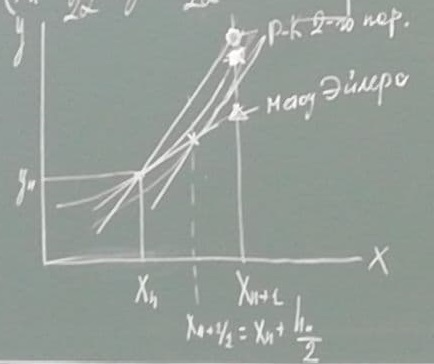
\includegraphics[scale=1.6]{a_1}}
	\caption{Геометрические результаты для a = 1}
\end{figure}

Рассмотрим для $\alpha = \frac{1}{2}$:\\
$y_{n+1} =  y_{n} + \frac{h_{n}}{2}[f(x_{n}, y_{n}) + f(x_{n} + \frac{h_{n}}{2}, y_{n} + \frac{h_{n}}{2} f (x_{n}, y_{n}))]$\\
1) $\overline{y_{n+1}} = y_{n} + h_{n} f(x_{n}, y_{n})$\\
2) $y'_{n+1} = f(x_{n} + h_{n}, \overline{y_{n+1}})$\\
3) $y'_{cp} = \frac{1}{2}(f(x_{n}, y_{n}) + y'_{n+ 1})$\\
4) $y_{n+1} = y_{n} + h_{n} \cdot y'_{cp}$
\begin{figure}[H]
	\center{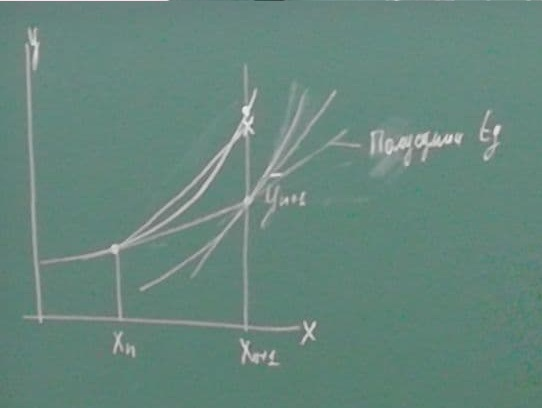
\includegraphics[scale=1.6]{a_2}}
	\caption{Геометрические результаты для a = 1/2}
\end{figure}


\section{Методы Рунге-Кутта 4-го порядка точности}
Формула обеспечивает переход из узла n в узлел n + 1:\\
$y_{n+1} = y_{n} + \frac{k_{1} + 2k_{2} + 2k_{3} + k_{4}}{6}$\\
$k_{1} = h f(x_{n}, y_{n})\\$
$k_{2} = h f (x_{n} + \frac{h}{2}, y_{n} + \frac{k_{1}}{2})$\\
$k_{2} = h f (x_{n} + \frac{h}{2}, y_{n} + \frac{k_{2}}{2})$\\
$k_{2} = h f (x_{n} + h, y_{n} + k_{3})$\\

Посмотрим, как формируется порядок точности в специальном варианте правой части:\\
$u'(x) = f(x)$\\
$y_{n+1} = y_{n} + \int\limits^{x_{n+1}}_{x_{n}}f(x) dx$\\
При $\alpha = \frac{1}{2}$\\
$y_{n+1} = y_{n} + \frac{h}{2}(f(x_{n}) + f(x_{n+1}))$\\
По методу трапеции:\\
$R_{trap} \leqslant \frac{x_{N} - x_{O}}{12} h^{2} \cdot max|f'(x)|$\\
Рунге-Кутт 4-го порядка:\\
$y_{n+1} = y_{n} + \frac{h}{6}(f(x_{n}) + 4f(x_{n} + \frac{h}{2}) + f(x_{n} + h))$ - метод Симпсона\\
$R_{simp} \leqslant \frac{x_{n} - x_{o}}{190 \cdot 16} h^{4} \cdot max|f^{IV}(x)|, x_{o} \leqslant x \leqslant x_{n}$\\

\section{Замечания о методах Рунге-Кутта}
\begin{enumerate}
\item методы явные - позволяет за строго зафиксированное количество шагов перейти из одного узла в другой
\item позволяет производить расчёты с переменным шагом
\item если нужных производынх при интегрировании нет, то применение метода Симпсона бессмысленно, т.е. метод трапеции, треугольника и тд.
\end{enumerate}

\section{Распространение метода Рунге-Кутта 4-то порядка на систему дифференциальных уравнений}
На примере метода Рунге-Кутта 4-го порядка рассмотрим распространить результат на систему дифференциальных уравнений.\\
\begin{equation}
\begin{cases}
u' = f(x, u, v)\\
v' = \phi(x, u, v)\\
u(\xi) = \eta_{1}\\
v(\xi) = \eta_{2}\\
\end{cases}
\end{equation}

$u = y, v = z$\\

$y_{n+1} = y_{n} + \frac{k_{1} + 2k_{2} + 2k_{3} + k_{4}}{6}$\\
$z_{n+1} = z_{n} + \frac{q_{1} + 2q_{2} + 2q_{3} + q_{4}}{6}$\\
$k_{1} = h f(x_{n}, y_{n}, z_{n}), q_{1} = h \phi(x_{n}, y_{n}, z_{n})$\\
$k_{2} = h f(x_{n} + \frac{h}{2}, y_{n} + \frac{k_{1}}{2}, z_{n} + \frac{q_{1}}{2}), q_{2} = h \phi(x_{n} + \frac{h}{2}, y_{n} + \frac{k_{1}}{2}, z_{n} + \frac{q_{1}}{2})$\\
$k_{3} = h f(x_{n} + \frac{h}{2}, y_{n} + \frac{k_{2}}{2}, z_{n} + \frac{q_{2}}{2}), q_{3} = h \phi(x_{n} + \frac{h}{2}, y_{n} + \frac{k_{2}}{2}, z_{n} + \frac{q_{2}}{2})$\\
$k_{4} = h f(x_{n} + \frac{h}{2}, y_{n} + \frac{k_{3}}{2}, z_{n} + \frac{q_{3}}{2}), q_{2} = h \phi(x_{n} + \frac{h}{2}, y_{n} + \frac{k_{3}}{2}, z_{n} + \frac{q_{3}}{2})$\\


Способ рассчёта выше применяется в вычислениях во второй лабораторной работе.\\

\section{Применение метода Пикара}
Возвращаясь к методу Пикара, сформулируем условие сходимости приближённого решения к точке.
\begin{itemize}
\item решение в ограниченной области
\item правая часть $f$ непрерывна
\item условия Липшеца: $a \leqslant x \leqslant b, |f(x, u_{1}) - f(x, u_{2})| \leqslant \mathcal{L}|u_{1} - u_{2}|$
\end{itemize}

\section{Неявный метод Эйлера}
$u' = f(x, u)$\\
В явном методе Эйлера - $y_{n+1} = y_{n} + h f(x_{n}, y_{n})$\\
В неявном методе Эйлера - $y_{n+1} = y_{n} + h f (x_{n + 1}, y_{n + 1})$
Последствия:\\
1) Решения может не быть, либо может быть несколько\\
2) Для решения уравнения необходимо подобрать метод\\
Применяется часто, поскольку является устойчивым.\\

Пример:\\
$u' = -\alpha u, \alpha > 0$\\
аналитическое решение: $u(x) = c e^{-\alpha x}$\\
\begin{figure}[H]
	\center{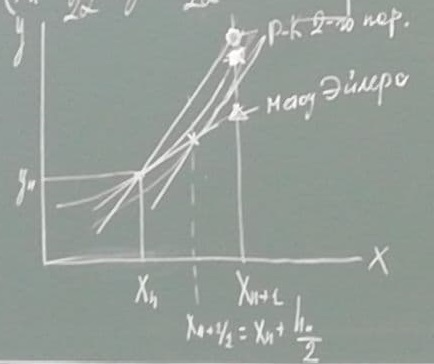
\includegraphics[scale=1.6]{a_1}}
	\caption{Сравнение явного и неявного метода Эйлера}
\end{figure}

$y_{n+1} = y_{n} - \alpha y_{n} h = y_{n} (1 - \alpha h), 1 - \alpha h > 0, h < \frac{1}{2}$\\
Применение явного метода может привести к расходящимся решениями и имеет ограничения на $\alpha$. Чем больше $\alpha$, тем больше шаг.\\

Неявный метод:\\
$y_{n+1} = y_{n} - \alpha y_{n+1}h$\\
$y_{n+1} = \frac{y_{n}}{1 + \alpha h}$ - ограничений на $h$ нет.\\

В общем виде:\\
$\sum\limits_{k=0}^{m} a_{k} y_{n - k} = h(f(x_{n}, y_{n}))$\\
$m = 1, a_{0} = 1, a_{1} = -1$\\
$y_{n} - y_{n - 1} = h f (x_{n}, y_{n})$ - метод Эйлера.\\

\section{Метод Гира}
При $m = 2$:\\
$\frac{3}{2} y_{n} - 2 y_{n-1} + \frac{1}{2}y_{n-2} = h f (x_{n}, y_{n}) + O(h^{2})$\\
При $m = 3$:\\
$\frac{11}{3}y_{n} - 3y_{n-1} + \frac{3}{2}y_{n-2} - \frac{1}{3}y_{n-3} = h f(x_{n}, y_{n}) + O(h^{3})$\\

Формул более высокого порядка точности не существует. Благоприятны с точки устойчивости решений.

\section{Замечание о многошаговых методах}
В многошаговых методах для получения решения в неизвестном узле необходимо знать значения в определённом количестве предыдущих узлов.

\section{Метод Адамса, 4-х шаговый, (p=4)}







